\documentclass{beamer}

\usetheme{CambridgeUS}
\setbeamertemplate{footline}[frame number] % Affiche uniquement le numéro de page

\setbeameroption{show notes on second screen=right} % Affiche les notes à droite
\usepackage[utf8]{inputenc}
\usepackage{graphicx}
\usepackage{hyperref}
\usepackage[T1]{fontenc}
\usepackage{caption}
\usepackage{placeins} % Required for \Floatbarrier

\title{Edge Computing: A Decentralized Evolution of the Cloud}
\author{Galiléa LE MOULLEC (Mun ID: 202415993) \and Félicien MOQUET (Mun ID: 202415994)}
\institute{Memorial University of Newfoundland, St. John's, Canada}
\date{March 2025}

\begin{document}

\begin{frame}
  \titlepage
\end{frame}

%--- Slide 1: Introduction ---
\begin{frame}{Introduction}
  \begin{itemize}
    \item Rapid growth of connected devices and real-time applications
    \item Traditional cloud computing reaches its limits
    \item \textbf{Edge computing} brings computation closer to the data source
  \end{itemize}
  \note{
    Over the past decade, we've seen an explosion of connected devices and services. Traditional cloud computing is showing its limits in terms of speed, privacy, and efficiency. Edge computing addresses these by bringing computation closer to where the data is generated.
  }
\end{frame}

%--- Slide 2: Why Edge Computing? ---
\begin{frame}{Why Edge Computing?}
  \begin{itemize}
    \item \textbf{Latency:} Reduces delay for real-time responses
    \item \textbf{Bandwidth:} Minimizes data transfer volume
    \item \textbf{Privacy:} Keeps sensitive data local
    \item \textbf{Resilience:} Operates even with cloud disconnections
  \end{itemize}
  \note{
    Edge computing helps reduce latency by processing data locally. It decreases bandwidth use, enhances privacy, and ensures services continue running even if the cloud is unavailable.
  }
\end{frame}

%--- Slide 3: Architecture Overview ---
\begin{frame}{Architecture Overview}
  \begin{itemize}
    \item \textbf{Edge devices:} Sensors, wearables, cameras
    \item \textbf{Edge nodes:} Gateways, micro-servers, local processors
    \item \textbf{Cloud layer:} For large-scale analytics and storage
  \end{itemize}
  \vspace{0.5cm}
  \centering
  \begin{figure}
    \centering
    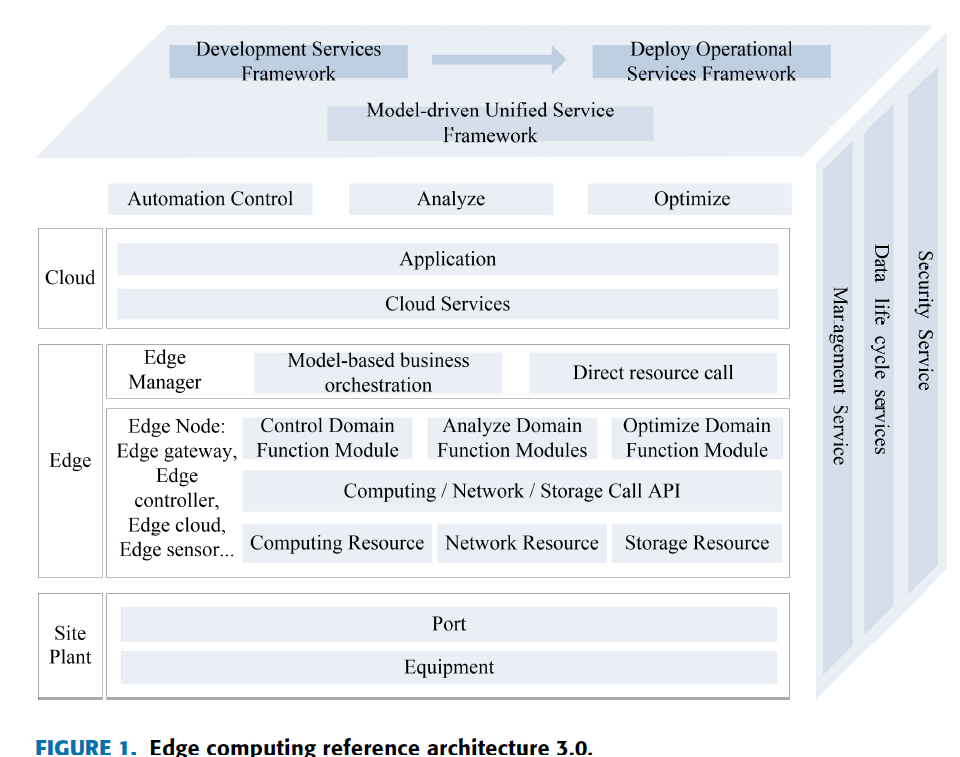
\includegraphics[width=0.5\linewidth]{IMG/6.png} % Optional
  \end{figure}

  \vspace{0.2cm}
  \small \textit{Figure 1: Edge computing reference architecture}

  \note{
    The edge architecture consists of three layers: edge devices, edge nodes, and the cloud. The goal is to shift part of the processing to the edge, while still leveraging cloud capabilities.
  }
\end{frame}

%--- Slide 4: Use Case - IoT ---
\begin{frame}{Use Case: Internet of Things (IoT)}
  \begin{itemize}
    \item Smart homes: temperature, lighting, security
    \item Environmental monitoring: air quality, agriculture
    \item Local processing improves responsiveness and privacy
  \end{itemize}
  \vspace{0.5cm}
  \centering
  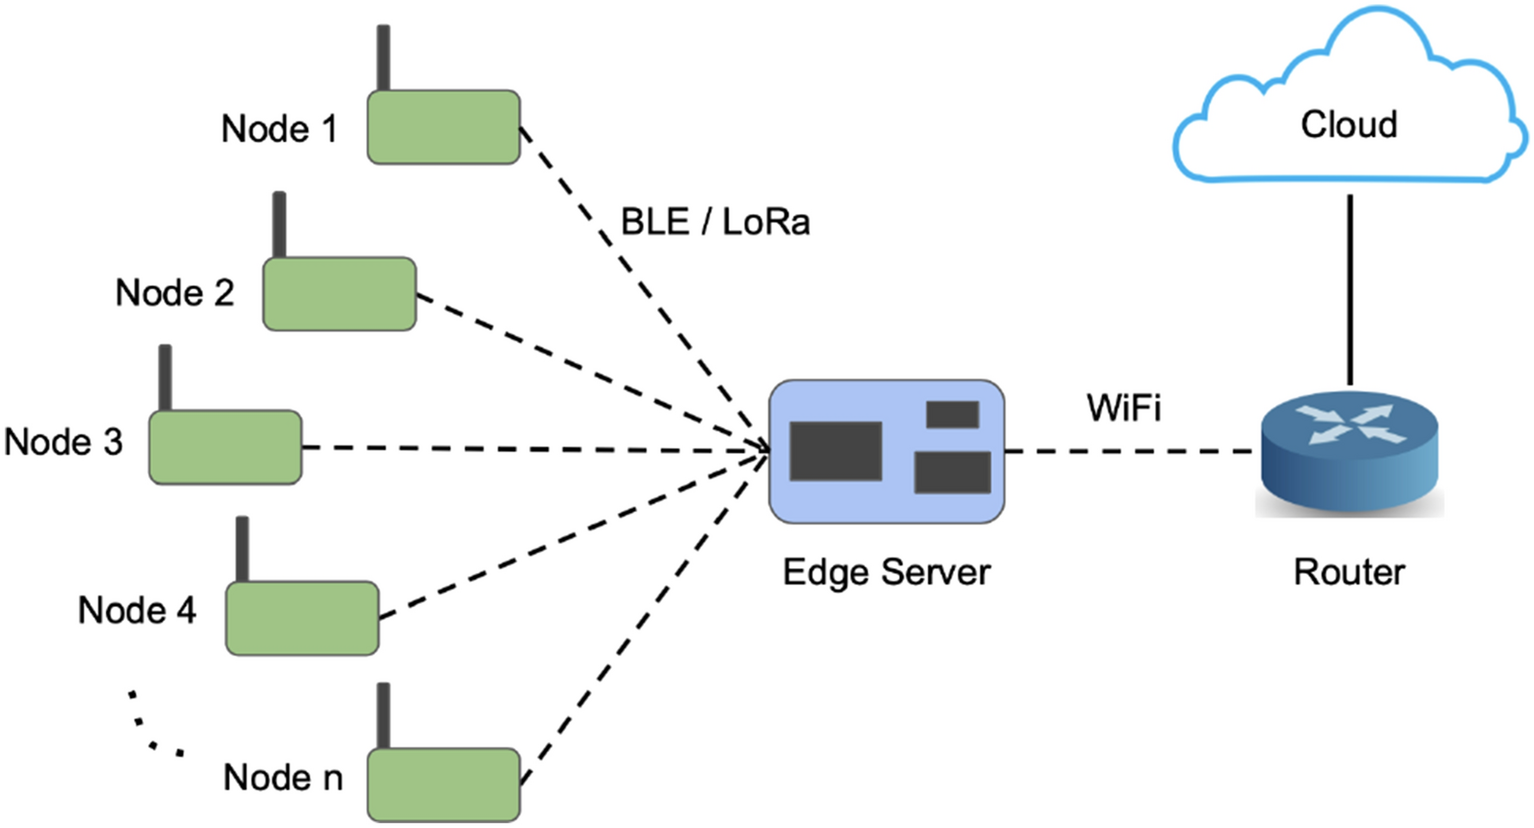
\includegraphics[width=0.6\linewidth]{IMG/12.png} % Optional
  \note{
    IoT applications benefit from edge computing through fast reactions and privacy. In smart homes, sensors react immediately. In agriculture, edge devices adapt irrigation in real time.
  }
\end{frame}

%--- Slide 5: Use Case - Autonomous Vehicles ---
\begin{frame}{Use Case: Autonomous Vehicles}
  \begin{itemize}
    \item Onboard sensors generate huge data streams
    \item Requires instant decision-making (e.g. braking)
    \item Edge computing enables safety-critical operations
  \end{itemize}
  \vspace{0.2cm}
  \centering
  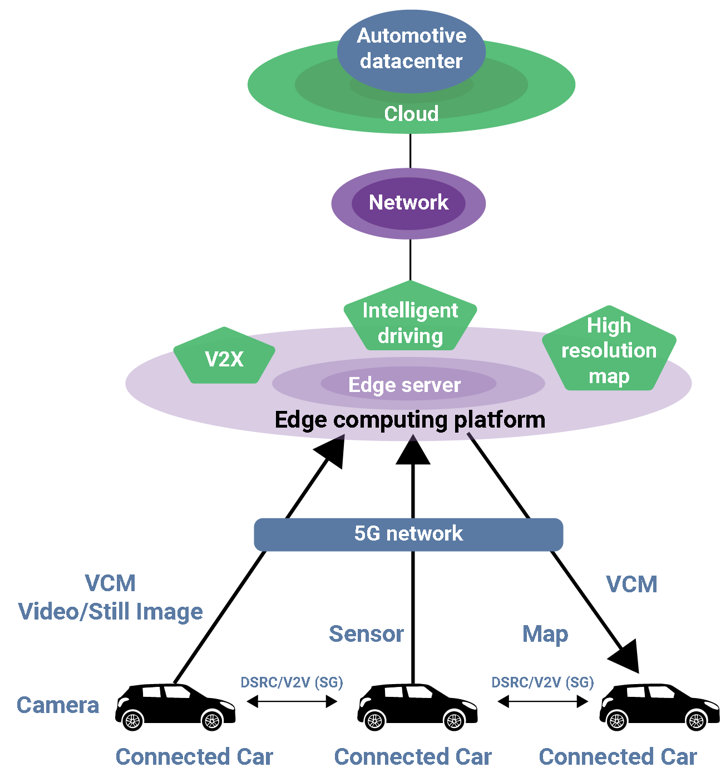
\includegraphics[width=0.05\linewidth]{IMG/13.png} % Optional
  \vspace{0.2cm}
  \small \textit{Figure 2: Smart homes architecture}
  \Floatbarrier
  \note{
    Autonomous vehicles need to process data within milliseconds. Edge computing allows cars to detect obstacles and make driving decisions instantly, which is essential for safety.
  }
\end{frame}

\begin{frame}{Use Case: Smart Cities}
    \begin{columns}[t]  % [t] pour aligner en haut
      % Colonne gauche : texte
      \begin{column}{0.5\textwidth}
        \begin{itemize}
          \item Real-time traffic management
          \item Public safety and surveillance
          \item Energy optimization and environmental monitoring
        \end{itemize}
      \end{column}
  
      % Colonne droite : image
      \begin{column}{0.5\textwidth}
        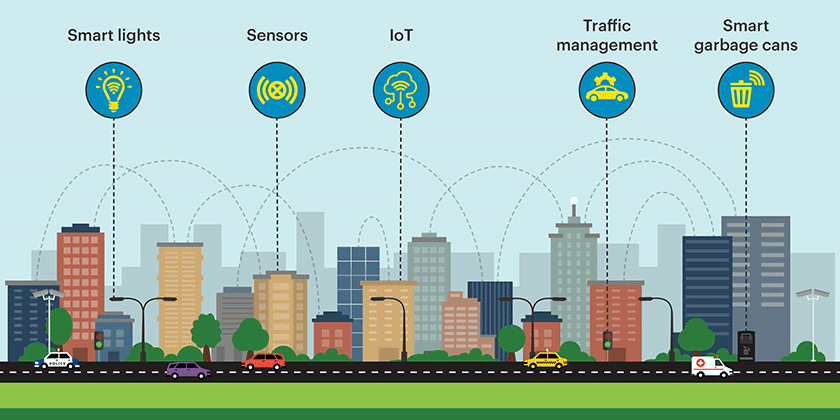
\includegraphics[width=\linewidth]{IMG/14.png}
        \vspace{0.2cm}
  
        \small \textit{Figure 4: Smart cities architecture}
      \end{column}
    \end{columns}
  
    \note{
      Edge computing enables cities to be smarter and more efficient. Local processing in traffic lights and surveillance systems improves responsiveness and reduces network dependency.
    }
  \end{frame}
  

%--- Slide 7: Use Case - Healthcare ---
\begin{frame}{Use Case: Healthcare and Telemedicine}
  \begin{itemize}
    \item Real-time patient monitoring
    \item On-site diagnostics in emergencies
    \item Strong data privacy and compliance (e.g. GDPR)
  \end{itemize}
  \vspace{0.5cm}
  \centering
  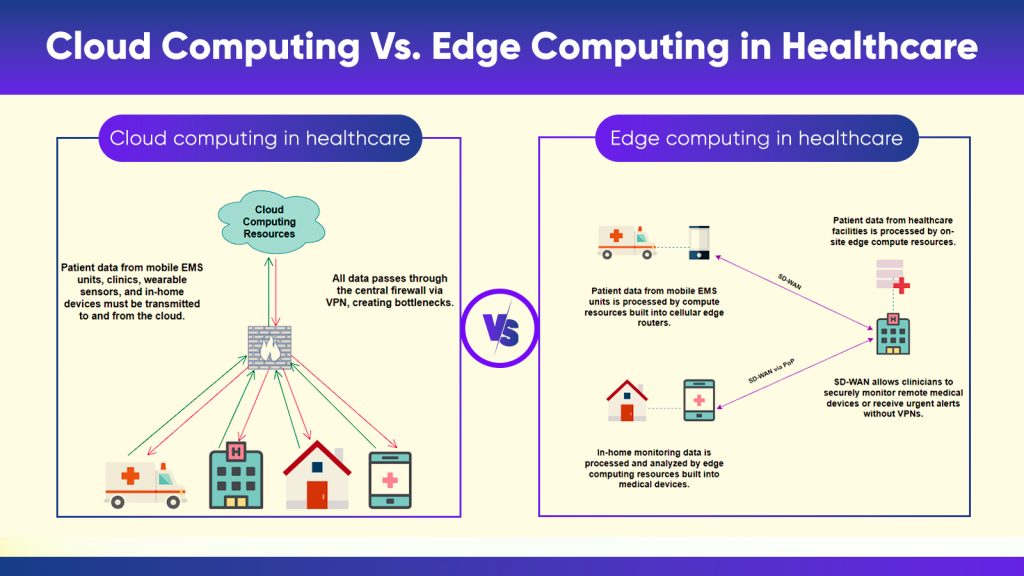
\includegraphics[width=0.6\linewidth]{IMG/15.jpg} % Optional
  \vspace{0.2cm}
  \small \textit{Figure 4: Edge computing reference architecture}
  \note{
    Healthcare systems use edge computing for real-time monitoring and diagnostics. Patient data stays local, enhancing privacy and compliance with health data regulations.
  }
\end{frame}

%--- Slide 8: Pros and Cons ---
\begin{frame}{Advantages and Challenges}
  \textbf{Advantages:}
  \begin{itemize}
    \item Lower latency and bandwidth usage
    \item Better data privacy and security
    \item Improved resilience and scalability
  \end{itemize}
  \vspace{0.3cm}
  \textbf{Challenges:}
  \begin{itemize}
    \item Complex management of distributed nodes
    \item Interoperability with cloud platforms
    \item Security at the edge
  \end{itemize}
  \note{
    While edge computing has many strengths, it introduces new challenges. Managing and securing distributed nodes is complex, and integration with existing cloud systems remains tricky.
  }
\end{frame}

%--- Slide 9: Trends and Future Perspectives ---
\begin{frame}{Trends and Future Perspectives}
  \begin{itemize}
    \item Integration with AI and 5G for smarter edge decisions
    \item Lightweight containers and orchestration (e.g. K3s)
    \item Research in privacy-preserving analytics, federated learning
  \end{itemize}
  \note{
    Edge computing is evolving. With AI, devices make smarter decisions. 5G supports high-speed communication. New tools like K3s make edge deployment easier, and research continues on privacy.
  }
\end{frame}

%--- Slide 10: Conclusion ---
\begin{frame}{Conclusion}
    \begin{itemize}
      \item Edge computing addresses key limitations of centralized cloud
      \item Use cases show strong benefits in latency, privacy, and efficiency
      \item Future: a hybrid cloud-edge ecosystem
    \end{itemize}
    \vspace{0.3cm}
    Thank you!
    \note{
      In conclusion, edge computing complements the cloud. It improves response times, protects data, and enables smarter systems. The future lies in combining both models for flexibility and power.
    }
  \end{frame}

%--- Slide 11: Open Question / Discussion ---
\begin{frame}{Open Discussion}
  \begin{block}{\textbf{Discussion Point}}
    Edge computing reduces data exchanges by processing locally. But:\\
    \textbf{With network demands constantly rising, will edge computing be enough?}\\
    Or is it just a temporary relief before a new saturation point?
  \end{block}
  \note{
    Let's open the floor: Do you think edge computing is a long-term solution, or just a short-term patch? Can it keep up with the exploding demand for connectivity and data?
  }
\end{frame}

%--- Slide 12: References---
\begin{frame}{References}
    \begin{itemize}
        \item \textit{Figure 1}: K. Cao, Y. Liu, G. Meng, et Q. Sun, «An Overview on Edge Computing Research», IEEE Access, vol. 8, p. 85714-85728, 2020, doi: 10.1109/ACCESS.2020.2991734.
        \item source 2
        \item ...
      \end{itemize}
\end{frame}

\end{document}
